\documentclass[a4paper,twoside]{article}
\usepackage{amssymb}
\usepackage{amsmath}
\usepackage{pgfplots}
\usepackage{tikz}
\usetikzlibrary{automata}
\usetikzlibrary{arrows}
\usetikzlibrary{shapes}
\usetikzlibrary{decorations.pathmorphing}

\begin{document}

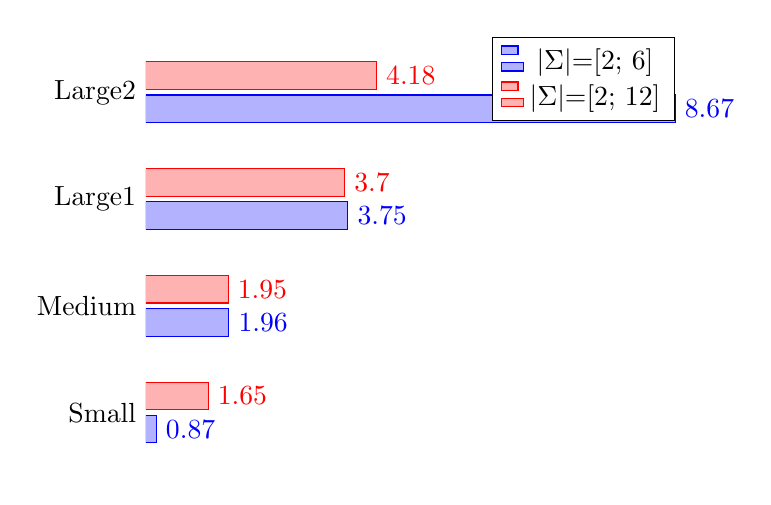
\begin{tikzpicture}
  \begin{axis}[%title  = Acceleration  per dataset,
   xbar,
    y axis line style = { opacity = 0 },
    axis x line       = none,
    tickwidth         = 0pt,
    enlarge y limits  = 0.2,
    enlarge x limits  = 0.02,
    symbolic y coords = {Small,Medium,Large1,Large2},
   nodes near coords,
  ]
 \addplot coordinates { (0.87,Small) (1.96,Medium)  (3.75,Large1)  (8.67,Large2)};
\addplot coordinates {  (3.7,Large1) (1.95,Medium)  (1.65,Small)
(4.18,Large2)};
\legend{$|\Sigma|$=[2; 6], $|\Sigma|$=[2; 12]}
\end{axis}
\end{tikzpicture}

\end{document}